\chapter[Leçon 33: Filmer, Kino a Medien]{Leçon 33: Virbereedung op de Sproochentest: Filmer, Kino a Medien \& Vokabelen a Grammaire}

Dës Lektioun ass eng geziilt Virbereedung op de mündleche Sproochentest fir d'Lëtzebuerger Nationalitéit zum Thema \textbf{Filmer, Kino a Medien}. Mir behandelen 12 zentral Froen an Äntwerten iwwer Kinos- a Televisiouns-Gewunnechten, Liblingsfilmer, Schauspiller a Medien-Evolutioun. Zousätzlech behandele mir wichteg Ausdréck a Verben aus dem Cours wéi \textbf{strampelen / eng Strampelbox}, \textbf{ophänken} (\textit{opgehaangen}), \textbf{ëmkippen} (\textit{ëmgekippt}), den Ënnerscheed tëscht \textbf{falen} an \textbf{ausfallen}, Ausdréck mat \textbf{schwaachfalen} (\textit{schwaachgefall}) a \textbf{sech verléiwen}, Grammaire-Formen an der 2. Persoun Singular (\textit{kanns de}, \textit{musst de}, \textit{wëllst de}) sou wéi d'Benotzung vum Verb \textbf{turnen}.

\textit{Cette leçon constitue une préparation ciblée à l'épreuve orale du Sproochentest pour l'obtention de la nationalité luxembourgeoise sur le thème \textbf{Films, cinéma et médias}. Nous traitons 12 questions et réponses clés concernant les habitudes d'écoute et de visionnage, les films préférés, les acteurs et l'évolution des médias. Nous abordons également des expressions et verbes importants du cours tels que \textbf{strampelen / eng Strampelbox} (gigoter/pédaler, salopette pour bébé), \textbf{ophänken} (accrocher, p.p. \textit{opgehaangen}), \textbf{ëmkippen} (renverser, p.p. \textit{ëmgekippt}), la différence entre \textbf{falen} (tomber) et \textbf{ausfallen} (être annulé / tomber en panne), des expressions avec \textbf{schwaachfalen} (\textit{schwaachgefall}) et \textbf{sech verléiwen}, les formes du présent à la 2e personne du singulier (\textit{kanns de}, \textit{musst de}, \textit{wëllst de}) ainsi que l'utilisation du verbe \textbf{turnen} (faire de la gymnastique/du sport).}

\textit{This lesson is a targeted preparation for the oral Sproochentest exam for Luxembourgish citizenship on the topic \textbf{Movies, Cinema, and Media}. We cover 12 core questions and answers regarding movie and TV habits, favorite films, actors, and media evolution. Additionally, we discuss key expressions and verbs from the lesson such as \textbf{strampelen / eng Strampelbox} (to kick/pedal, baby romper), \textbf{ophänken} (to hang up, p.p. \textit{opgehaangen}), \textbf{ëmkippen} (to tip over/spill, p.p. \textit{ëmgekippt}), the difference between \textbf{falen} (to fall) and \textbf{ausfallen} (to be cancelled / to break down), expressions with \textbf{schwaachfalen} (\textit{schwaachgefall}) and \textbf{sech verléiwen}, 2nd-person singular grammar forms (\textit{kanns de}, \textit{musst de}, \textit{wëllst de}), as well as the verb \textbf{turnen} (to do gymnastics/sports).}

\vspace{1.5em}

\section[Wichteg Ausdréck a Verben / Key Verbs \& Expressions]{Wichteg Ausdréck a Verben aus dem Cours \\/ Expressions et verbes clés du cours \\/ Key Expressions and Verbs from the Lesson}

\subsection*{1. strampelen (strampelt / gestrampelt) \& eng Strampelbox}

\noindent\textit{Français : Gigoter des pieds, pédaler énergiquement (pour un bébé ou à vélo). Une \textbf{Strampelbox} (f.) désigne une salopette ou grenouillère pour bébé.}\\
\textit{English: To kick one's feet, pedal energetically (for a baby or on a bicycle). A \textbf{Strampelbox} (f.) refers to a baby romper / overalls.}

\begin{itemize}
    \item \textbf{Beispill 1 (Bébé / Baby):} \textit{De Puppelchen läit am Bett a strampelt mat de Been.}\\
    $\rightarrow$ Français : \textit{Le bébé est couché dans le lit et gigote avec ses jambes.}\\
    $\rightarrow$ English : \textit{The baby lies in bed and kicks its legs.}
    
    \item \textbf{Beispill 2 (Vëlo / Bicycle):} \textit{Ech muss séier um Vëlo strampelen fir pünktlech ze kommen.}\\
    $\rightarrow$ Français : \textit{Je dois pédaler vite à vélo pour arriver à l'heure.}\\
    $\rightarrow$ English : \textit{I have to pedal fast on the bicycle to arrive on time.}
    
    \item \textbf{Beispill 3 (Strampelbox / Baby romper):} \textit{D'Mamm keeft eng nei wäermer Strampelbox fir de Wanter.}\\
    $\rightarrow$ Français : \textit{La mère achète une nouvelle salopette plus chaude pour l'hiver.}\\
    $\rightarrow$ English : \textit{The mother buys a new warmer baby romper for the winter.}
\end{itemize}

\subsection*{2. ophänken (hänkt op / aufgehaangen, aufgehaang)}

\noindent\textit{Français : Accrocher, suspendre au mur (un tableau, un miroir, un cadre). Participe passé : \textbf{opgehaangen} ou \textbf{opgehaang}.}\\
\textit{English: To hang up, suspend on the wall (a picture, a mirror, a frame). Past participle: \textbf{opgehaangen} or \textbf{opgehaang}.}

\begin{itemize}
    \item \textbf{Beispill:} \textit{Ech hänken e schéint Bild an e Spigel am Living op. Mir hunn d'Fotoen schonn aufgehaangen.}\\
    $\rightarrow$ Français : \textit{J'accroche un beau tableau et un miroir dans le séjour. Nous avons déjà accroché les photos.}\\
    $\rightarrow$ English : \textit{I hang up a beautiful picture and a mirror in the living room. We have already hung up the photos.}
\end{itemize}

\subsection*{3. ëmkippen (kippt ëm / ëmgekippt)}

\noindent\textit{Français : Renverser, faire basculer un objet posé verticalement (un verre, une bouteille, un vase). Participe passé : \textbf{ëmgekippt}. À ne pas confondre avec « falen » (tomber de haut).}\\
\textit{English: To tip over, spill, knock over an upright object (a glass, a bottle, a vase). Past participle: \textbf{ëmgekippt}. Not to be confused with "falen" (falling down from height).}

\begin{itemize}
    \item \textbf{Beispill:} \textit{Ech hunn aus Verseeën de Glas Wäin um Dësch ëmgekippt.}\\
    $\rightarrow$ Français : \textit{J'ai renversé par mégarde le verre de vin sur la table.}\\
    $\rightarrow$ English : \textit{I accidentally knocked over the glass of wine on the table.}
\end{itemize}

\subsection*{4. falen vs. ausfallen a wichtege Ausdréck}

\noindent\textit{Français : \textbf{falen} signifie tomber. \textbf{ausfallen} signifie être annulé (un cours, un rendez-vous) ou tomber en panne / être interrompu (le courant, l'électricité).}\\
\textit{English: \textbf{falen} means to fall. \textbf{ausfallen} means to be cancelled (a lesson, an event) or to break down / go out (power, electricity).}

\begin{itemize}
    \item \textbf{ausfallen (Annulation / Panne):} \textit{De nächste Lëtzebuerger Kurs fällt aus, well de Enseignant krank ass. De Stroum ass gëschter den Owend ausgefall.}\\
    $\rightarrow$ Français : \textit{Le prochain cours de luxembourgeois est annulé parce que l'enseignant est malade. Le courant a sauté hier soir.}\\
    $\rightarrow$ English : \textit{The next Luxembourgish lesson is cancelled because the teacher is sick. The power went out yesterday evening.}
    
    \item \textbf{eng Pann hunn (Panne de voiture / Breakdown):} \textit{Mäin Auto geet net méi un, ech hunn eng Pann um Wee fir op d'Aarbecht.}\\
    $\rightarrow$ Français : \textit{Ma voiture ne démarre plus, j'ai une panne sur le chemin du travail.}\\
    $\rightarrow$ English : \textit{My car won't start, I have a breakdown on the way to work.}
    
    \item \textbf{Malaise \& S'évanouir (schwaachfalen / schwaachgefall):}
    \begin{itemize}
        \item \textit{schwaachfalen (fällt schwaach / schwaachgefall):} \textit{Hien ass gëschter schwaachgefall.} (Il s'est évanoui hier. / He fainted yesterday.)
        \item \textit{Mir ass schwindeleg / schwammeg am Kapp ginn.} (J'ai eu le tournis / la tête qui tourne. / I felt dizzy / lightheaded.)
    \end{itemize}
    
    \item \textbf{sech verléiwen vs. verléift sinn:}
    \begin{itemize}
        \item \textit{sech verléiwen (an een)} = Tomber amoureux (de quelqu'un) / To fall in love (with someone).
        \item \textit{verléift sinn} = Être amoureux / To be in love.
        \item \textit{Beispill:} \textit{Si hunn sech séier verléift a si sinn elo ganz verléift.} (Ils sont vite tombés amoureux et sont très amoureux maintenant. / They fell in love quickly and are very much in love now.)
    \end{itemize}
\end{itemize}

\subsection*{5. Grammaire: Formen an der 2. Persoun Singular (2nd Person Singular Forms)}

\noindent\textit{Français : En luxembourgeois, la terminaison de la 2e personne du singulier pour ces verbes se termine naturellement en \textbf{-s} / \textbf{-lls} / \textbf{-ss} (\textit{du kanns}, \textit{du muss}, \textit{du wëlls}, \textit{du méchs}).}\\
\textit{English: In Luxembourgish, the 2nd person singular form for these verbs ends naturally in \textbf{-s} / \textbf{-lls} / \textbf{-ss} (\textit{du kanns}, \textit{du muss}, \textit{du wëlls}, \textit{du méchs}).}

\begin{itemize}
    \item \textbf{kënnen (pouvoir / can):} \textit{Du kanns} / \textit{Kanns de dat maachen?} (Peux-tu faire cela ? / Can you do that?)
    \item \textbf{müssen (devoir / must):} \textit{Du muss} / \textit{Muss de haut schaffen?} (Dois-tu travailler aujourd'hui ? / Do you have to work today?)
    \item \textbf{wëllen (vouloir / want):} \textit{Du wëlls} / \textit{Wëllst de an de Kino goen?} (Veux-tu aller au cinéma ? / Do you want to go to the cinema?)
    \item \textbf{maachen (faire / do, make):} \textit{Du méchs} / \textit{Méchs de de Sport?} (Fais-tu du sport ? / Do you do sports?)
\end{itemize}

\subsection*{6. turnen / tournen (Faire de la gymnastique, du sport / Gymnastics, sports)}

\noindent\textit{Français : Le verbe \textbf{turnen} désigne la gymnastique ou les exercices physiques généraux.}\\
\textit{English: The verb \textbf{turnen} refers to doing gymnastics or physical workouts.}

\begin{itemize}
    \item \textbf{Beispill:} \textit{Ech ginn all Donneschdeg Owend am Sportscenter turnen.}\\
    $\rightarrow$ Français : \textit{Je vais faire de la gymnastique/du sport tous les jeudis soir au centre sportif.}\\
    $\rightarrow$ English : \textit{I go to do gymnastics/sports every Thursday evening at the sports center.}
\end{itemize}

\vspace{1.5em}

\section[Sproochentest Deel 1: Filmer, Kino a Medien / Q\&A]{Sproochentest Deel 1: Filmer, Kino a Medien \\/ Questions et réponses : Films, cinéma et médias \\/ Questions and Answers: Movies, Cinema, and Media}

\noindent\textbf{1. Gitt Dir gär an de Kino? Wéi oft gitt Dir an de Kino?}\\
\textit{(FR: Allez-vous volontiers au cinéma ? À quelle fréquence y allez-vous ? — EN: Do you like going to the cinema? How often do you go to the cinema?)}\\[0.3em]
\textit{Jo, ech ginn iergendwéi gär an de Kino, mä net ganz oft. Ech ginn ongeféier zwee- bis dräimol d'Joer an de Kino, meeschtens am Wanter.}\\
\textit{Jo} (Oui / Yes), \textit{ech ginn} (je vais / I go) \textit{iergendwéi gär} (plutôt volontiers, d'une certaine manière / sort of enjoyably) \textit{an de Kino} (au cinéma / to the cinema), \textit{mä net ganz oft} (mais pas très souvent / but not very often). \textit{Ech ginn} (Je vais / I go) \textit{ongeféier} (environ / approximately) \textit{zwee- bis dräimol d'Joer} (deux à trois fois par an / two to three times a year) \textit{an de Kino} (au cinéma / to the cinema), \textit{meeschtens am Wanter} (la plupart du temps en hiver / mostly in winter).\\
$\rightarrow$ Français : \textit{Oui, j'aime bien aller au cinéma, mais pas très souvent. J'y vais environ deux à trois fois par an, la plupart du temps en hiver.}\\
$\rightarrow$ English : \textit{Yes, I like going to the cinema, but not very often. I go about two to three times a year, mostly in winter.}\\[0.8em]

\noindent\textbf{2. Firwat gitt Dir gär (oder net gär) an de Kino?}\\
\textit{(FR: Pourquoi aimez-vous (ou n'aimez-vous pas) aller au cinéma ? — EN: Why do you like (or dislike) going to the cinema?)}\\[0.3em]
\textit{Ech ginn gär an de Kino, well d'Leinwand ganz grouss ass, de Sound super ass, an et ass en agreablen Entspannungsmoment. Wat mir manner gefällt ass, datt den Ticket an d'Popcorn zimmlech deier sinn.}\\
\textit{Ech ginn gär} (J'aime aller / I like going) \textit{an de Kino} (au cinéma / to the cinema), \textit{well d'Leinwand} (parce que l'écran géant / because the screen) \textit{ganz grouss ass} (est très grand / is very big), \textit{de Sound} (le son / the sound) \textit{super ass} (est super / is great), \textit{an et ass} (et c'est / and it is) \textit{en agreablen Entspannungsmoment} (un moment de détente agréable / a pleasant relaxation moment). \textit{Wat mir manner gefällt} (Ce qui me plaît moins / What I like less) \textit{ass, datt den Ticket} (est que le billet / is that the ticket) \textit{an d'Popcorn} (et le popcorn / and popcorn) \textit{zimmlech deier sinn} (sont assez chers / are quite expensive).\\
$\rightarrow$ Français : \textit{J'aime aller au cinéma parce que le grand écran et le son sont supers, et c'est un moment de détente agréable. Ce qui me plaît moins, c'est que le billet et le popcorn sont assez chers.}\\
$\rightarrow$ English : \textit{I like going to the cinema because the big screen and the sound are great, and it's a pleasant relaxation moment. What I like less is that the ticket and popcorn are quite expensive.}\\[0.8em]

\noindent\textbf{3. Wat fir eng Zort Filmer kuckt Dir am léifsten?}\\
\textit{(FR: Quel genre de films regardez-vous de préférence ? — EN: What kind of movies do you like to watch most?)}\\[0.3em]
\textit{Ech kucken am léifsten Komedien, Actionfilmer a Dokumentarfilmer. Ech kucken guer net gär Horrorfilmer, well si mir ze vill Angscht maachen!}\\
\textit{Ech kucken} (Je regarde / I watch) \textit{am léifsten} (de préférence / most of all) \textit{Komedien} (des comédies / comedies), \textit{Actionfilmer} (des films d'action / action movies) \textit{a Dokumentarfilmer} (et des documentaires / and documentaries). \textit{Ech kucken guer net gär} (Je n'aime pas du tout regarder / I don't at all like watching) \textit{Horrorfilmer} (des films d'horreur / horror movies), \textit{well si mir} (parce qu'ils me / because they) \textit{ze vill Angscht maachen} (font trop peur / make me too scared)!\\
$\rightarrow$ Français : \textit{Je regarde de préférence des comédies, des films d'action et des documentaires. Je n'aime pas du tout regarder les films d'horreur parce qu'ils me font trop peur !}\\
$\rightarrow$ English : \textit{I prefer watching comedies, action films, and documentaries. I don't like watching horror movies at all because they scare me too much!}\\[0.8em]

\noindent\textbf{4. Wat ass Ären absolutten Liblingsfilm? Erzielt eng kuerz Geschicht dovun.}\\
\textit{(FR: Quel est votre film préféré ? Racontez brièvement son histoire. — EN: What is your favorite movie? Tell a short summary of its story.)}\\[0.3em]
\textit{Mäi Liblingsfilm ass « Shrek ». Dat ass de Sujet vun engem gréngen Oger, deen eleng an enger Supp lieft. Hie mécht eng Rees fir seng Rou ze erhuelen a verléift sech an eng Prinzessin. Et ass e ganz amüsanten a schéinen Zeechentrickfilm.}\\
\textit{Mäi Liblingsfilm} (Mon film préféré / My favorite movie) \textit{ass « Shrek »}. \textit{Dat ass de Sujet} (C'est le sujet, l'histoire / That is the topic/story) \textit{vun engem gréngen Oger} (d'un ogre vert / of a green ogre) \textit{deen eleng} (qui seul / who alone) \textit{an enger Supp lieft} (vit dans un marais / lives in a swamp). \textit{Hie mécht eng Rees} (Il fait un voyage / He makes a journey) \textit{fir seng Rou ze erhuelen} (pour retrouver sa tranquillité / to get his peace back) \textit{a verléift sech} (et tombe amoureux / and falls in love) \textit{an eng Prinzessin} (d'une princesse / with a princess). \textit{Et ass} (C'est / It is) \textit{e ganz amüsanten a schéinen Zeechentrickfilm} (un dessin animé très amusant et beau / a very amusing and beautiful animated movie).\\
$\rightarrow$ Français : \textit{Mon film préféré est « Shrek ». C'est l'histoire d'un ogre vert qui vit seul dans un marais. Il entreprend un voyage pour retrouver sa tranquillité et tombe amoureux d'une princesse. C'est un dessin animé très amusant et beau.}\\
$\rightarrow$ English : \textit{My favorite movie is "Shrek". It's the story of a green ogre who lives alone in a swamp. He goes on a journey to regain his peace and falls in love with a princess. It's a very amusing and beautiful animated movie.}\\[0.8em]

\noindent\textbf{5. Wat ass den Ënnerscheed tëscht de Filmer am Kino a Filmer doheem op Netflix kucken?}\\
\textit{(FR: Quelle est la différence entre regarder des films au cinéma et à la maison sur Netflix ? — EN: What is the difference between watching movies at the cinema and at home on Netflix?)}\\[0.3em]
\textit{Doheem op Netflix kënne mir kucken wéini mir wëllen, mir kënnen eng Paus maachen a mir sinn bequem um Canapé. Mä am Kino ass d'Atmosphär an d'Kinoserfahrung vill méi spektakulär.}\\
\textit{Doheem op Netflix} (À la maison sur Netflix / At home on Netflix) \textit{kënne mir kucken} (nous pouvons regarder / we can watch) \textit{wéini mir wëllen} (quand nous voulons / whenever we want), \textit{mir kënnen eng Paus maachen} (nous pouvons faire une pause / we can take a break) \textit{a mir sinn bequem} (et nous sommes confortablement installés / and we are comfortable) \textit{um Canapé} (sur le canapé / on the couch). \textit{Mä am Kino} (Mais au cinéma / But at the cinema) \textit{ass d'Atmosphär} (l'atmosphère est / the atmosphere is) \textit{an d'Kinoserfahrung} (et l'expérience cinéma / and the cinema experience) \textit{vill méi spektakulär} (beaucoup plus spectaculaire / much more spectacular).\\
$\rightarrow$ Français : \textit{À la maison sur Netflix, nous pouvons regarder quand nous voulons, faire une pause et être confortables sur le canapé. Mais au cinéma, l'atmosphère et l'expérience sont bien plus spectaculaires.}\\
$\rightarrow$ English : \textit{At home on Netflix we can watch whenever we want, pause, and be comfortable on the couch. But at the cinema the atmosphere and cinematic experience are much more spectacular.}\\[0.8em]

\noindent\textbf{6. Hutt Dir e Liblingsschauspiller oder eng Liblingsschauspillerin?}\\
\textit{(FR: Avez-vous un acteur ou une actrice préféré(e) ? — EN: Do you have a favorite actor or actress?)}\\[0.3em]
\textit{Mäi Liblingsschauspiller ass de Christian Bale. Hien ass e ganz fantastesche Schauspiller, well hie seng Rollen ëmmer mat vill Leidenschaft an Dedikatioun spillt.}\\
\textit{Mäi Liblingsschauspiller} (Mon acteur préféré / My favorite actor) \textit{ass de Christian Bale}. \textit{Hien ass} (Il est / He is) \textit{e ganz fantastesche Schauspiller} (un acteur très fantastique / a very fantastic actor), \textit{well hie seng Rollen} (parce qu'il ses rôles / because he his roles) \textit{ëmmer} (toujours / always) \textit{mat vill Leidenschaft an Dedikatioun spillt} (joue avec beaucoup de passion et de dévouement / plays with a lot of passion and dedication).\\
$\rightarrow$ Français : \textit{Mon acteur préféré est Christian Bale. C'est un fantastique acteur parce qu'il joue toujours ses rôles avec beaucoup de passion et d'engagement.}\\
$\rightarrow$ English : \textit{My favorite actor is Christian Bale. He is a fantastic actor because he always plays his roles with a lot of passion and dedication.}\\[0.8em]

\noindent\textbf{7. Kuckt Dir gär Neiegkeeten (Noriichten) oder Dokumentarfilmer op der Tëlee?}\\
\textit{(FR: Regardez-vous la télévision, les informations ou les documentaires ? — EN: Do you like watching the news or documentaries on TV?)}\\[0.3em]
\textit{Ech kucken net vill klassesch Tëlee, mä ech kucken d'Neiegkeeten um Handy oder um Internet, an ech kucke gär Dokumentarfilmer iwwer d'Natur a Geschicht op Arte.}\\
\textit{Ech kucken net vill} (Je ne regarde pas beaucoup de / I don't watch much) \textit{klassesch Tëlee} (télévision classique / classical TV), \textit{mä ech kucken} (mais je regarde / but I watch) \textit{d'Neiegkeeten} (les informations, nouvelles / the news) \textit{um Handy oder um Internet} (sur le téléphone portable ou sur internet / on the smartphone or internet), \textit{an ech kucke gär} (et j'aime regarder / and I like watching) \textit{Dokumentarfilmer} (des documentaires / documentaries) \textit{iwwer d'Natur a Geschicht} (sur la nature et l'histoire / about nature and history) \textit{op Arte} (sur Arte / on Arte).\\
$\rightarrow$ Français : \textit{Je ne regarde pas beaucoup la télévision classique, mais je consulte les nouvelles sur smartphone ou sur internet, et j'aime regarder des documentaires sur la nature et l'histoire sur Arte.}\\
$\rightarrow$ English : \textit{I don't watch much traditional TV, but I check the news on my smartphone or the internet, and I like watching documentaries about nature and history on Arte.}\\[0.8em]

\noindent\textbf{8. Wéi hutt Dir fréier Filmer gekuckt: mat Video-Kassetten, DVDen oder Streaming?}\\
\textit{(FR: Comment regardiez-vous des films autrefois : avec des cassettes vidéo, des DVD ou en streaming ? — EN: How did you watch movies in the past: with video cassettes, DVDs, or streaming?)}\\[0.3em]
\textit{Fréier hu mir Video-Kassetten mat engem Videorekorder gekuckt a mir hunn DVDen an der Videothéik geléint. Haut kucke mir bal alles direkt op Streaming-Platformen.}\\
\textit{Fréier} (Autrefois, auparavant / In the past, previously) \textit{hu mir gekuckt} (nous avons regardé / we watched) \textit{Video-Kassetten} (des cassettes vidéo / video cassettes) \textit{mat engem Videorekorder} (avec un magnétoscope / with a VCR) \textit{a mir hunn geléint} (et nous avons loué / and we rented) \textit{DVDen} (des DVD / DVDs) \textit{an der Videothéik} (au vidéoclub / at the video store). \textit{Haut kucke mir} (Aujourd'hui nous regardons / Today we watch) \textit{bal alles} (presque tout / almost everything) \textit{direkt op Streaming-Platformen} (directement sur les plateformes de streaming / directly on streaming platforms).\\
$\rightarrow$ Français : \textit{Autrefois, nous regardions des cassettes vidéo avec un magnétoscope et nous louions des DVD au vidéoclub. Aujourd'hui, nous regardons presque tout directement sur les plateformes de streaming.}\\
$\rightarrow$ English : \textit{In the past, we watched video cassettes with a VCR and rented DVDs at the video rental store. Today, we watch almost everything directly on streaming platforms.}\\[0.8em]

\noindent\textbf{9. Kuckt Dir Filmer op Franséisch, Englesch oder mat Ënnertitelen?}\\
\textit{(FR: Regardez-vous les films en français, en anglais ou avec des sous-titres ? — EN: Do you watch movies in French, English, or with subtitles?)}\\[0.3em]
\textit{Ech kucken d'Filmer meeschtens op Englesch am Original mat Franséischen oder Engleschen Ënnertitelen. Heiansdo kucken ech och Filmer op Franséisch.}\\
\textit{Ech kucken} (Je regarde / I watch) \textit{d'Filmer} (les films / movies) \textit{meeschtens} (la plupart du temps / mostly) \textit{op Englesch} (en anglais / in English) \textit{am Original} (en version originale / in original version) \textit{mat Franséischen oder Engleschen Ënnertitelen} (avec des sous-titres français ou anglais / with French or English subtitles). \textit{Heiansdo} (Parfois / Sometimes) \textit{kucken ech och} (je regarde aussi / I also watch) \textit{Filmer op Franséisch} (des films en français / movies in French).\\
$\rightarrow$ Français : \textit{Je regarde la plupart du temps les films en anglais en version originale avec des sous-titres français ou anglais. Parfois, je regarde aussi des films en français.}\\
$\rightarrow$ English : \textit{Most of the time I watch movies in English in original version with French or English subtitles. Sometimes I also watch movies in French.}\\[0.8em]

\noindent\textbf{10. Gitt Dir léiwer aleng oder mat Frënn a Famill an de Kino?}\\
\textit{(FR: Préférez-vous aller au cinéma seul(e) ou avec des amis et la famille ? — EN: Do you prefer going to the cinema alone or with friends and family?)}\\[0.3em]
\textit{Ech ginn meeschtens mat menger Famill oder mat menge Frënn an de Kino, well mir no dem Film gär an e Restaurant ginn an iwwer de Film diskutéieren.}\\
\textit{Ech ginn meeschtens} (Je vais généralement / I usually go) \textit{mat menger Famill} (avec ma famille / with my family) \textit{oder mat menge Frënn} (ou avec mes amis / or with my friends) \textit{an de Kino} (au cinéma / to the cinema), \textit{well mir} (parce que nous / because we) \textit{no dem Film} (après le film / after the movie) \textit{gär an e Restaurant ginn} (aimons aller au restaurant / like going to a restaurant) \textit{an iwwer de Film diskutéieren} (et discuter du film / and discuss the movie).\\
$\rightarrow$ Français : \textit{Je vais généralement au cinéma avec ma famille ou avec mes amis, parce qu'après le film nous aimons aller au restaurant et discuter du film.}\\
$\rightarrow$ English : \textit{I usually go to the cinema with my family or with my friends, because after the movie we like to go to a restaurant and discuss the film.}\\[0.8em]

\noindent\textbf{11. Kuckt Dir léiwer Serien oder Spillfilmer?}\\
\textit{(FR: Préférez-vous regarder des séries ou des longs métrages ? — EN: Do you prefer watching TV series or feature films?)}\\[0.3em]
\textit{Dat hänkt vun der Zäit of: während der Woch kucken ech gär eng kuerz Episode vun enger Serie, mä am Weekend kucken ech léiwer e ganze Spillfilm.}\\
\textit{Dat hänkt... of} (Cela dépend / That depends) \textit{vun der Zäit} (du temps / on time): \textit{während der Woch} (pendant la semaine / during the week) \textit{kucken ech gär} (j'aime regarder / I like watching) \textit{eng kuerz Episode} (un bref épisode / a short episode) \textit{vun enger Serie} (d'une série / of a series), \textit{mä am Weekend} (mais le week-end / but on the weekend) \textit{kucken ech léiwer} (je préfère regarder / I prefer watching) \textit{e ganze Spillfilm} (un long métrage entier / a full feature film).\\
$\rightarrow$ Français : \textit{Cela dépend du temps disponible : pendant la semaine, j'aime regarder un court épisode de série, mais le week-end, je préfère regarder un long métrage entier.}\\
$\rightarrow$ English : \textit{That depends on available time: during the week I like watching a short series episode, but on weekends I prefer watching a full feature film.}\\[0.8em]

\noindent\textbf{12. Wéi vill Zäit verbréngt Är Famill virun de Schiermer (Handy, Tëlee, Tablet)?}\\
\textit{(FR: Combien de temps votre famille passe-t-elle devant les écrans (smartphone, télé, tablette) ? — EN: How much time does your family spend in front of screens (smartphone, TV, tablet)?)}\\[0.3em]
\textit{Mir probéieren d'Zäit virun de Schiermer ze limitéieren, besonnesch fir d'Kanner. Am Owend kucken mir heiansdo zesummen e schéine Familljefilm.}\\
\textit{Mir probéieren} (Nous essayons de / We try to) \textit{d'Zäit} (le temps / time) \textit{virun de Schiermer} (devant les écrans / in front of screens) \textit{ze limitéieren} (de limiter / to limit), \textit{besonnesch fir d'Kanner} (particulièrement pour les enfants / especially for the children). \textit{Am Owend} (Le soir / In the evening) \textit{kucken mir heiansdo} (nous regardons parfois / we sometimes watch) \textit{zesummen} (ensemble / together) \textit{e schéine Familljefilm} (un beau film de famille / a nice family movie).\\
$\rightarrow$ Français : \textit{Nous essayons de limiter le temps passé devant les écrans, particulièrement pour les enfants. Le soir, nous regardons parfois un beau film en famille.}\\
$\rightarrow$ English : \textit{We try to limit screen time, especially for the children. In the evening, we sometimes watch a nice family film together.}

\vspace{1.5em}

\section[Vokabelen: Filmer, Kino a Medien / Vocabulary Table]{Vokabelen: Filmer, Kino a Medien \\/ Vocabulaire : Films, cinéma et médias \\/ Vocabulary: Movies, Cinema, and Media}

\begin{table}[h!]
\centering
\small
\begin{tabular}{p{3.5cm}p{3.2cm}p{4.0cm}p{4.0cm}}
\toprule
\textbf{Lëtzebuergesch} & \textbf{Plural} & \textbf{Français} & \textbf{English} \\
\midrule
de Kino & d'Kinoen & le cinéma & cinema / movie theater \\
de Film & de Filmer & le film & movie / film \\
de Liblingsfilm & de Liblingsfilmer & le film préféré & favorite movie \\
d'Komedie & d'Komedien & la comédie & comedy \\
den Actionfilm & den Actionfilmer & le film d'action & action movie \\
den Horrorfilm & den Horrorfilmer & le film d'horreur & horror movie \\
de Dokumentarfilm & de Dokumentarfilmer & le documentaire & documentary \\
de Zeechentrickfilm & de Zeechentrickfilmer & le dessin animé & animated film / cartoon \\
d'Drama & d'Dramaen & le drame & drama \\
de Sci-Fi Film & de Sci-Fi Filmer & le film de science-fiction & sci-fi movie \\
de Schauspiller & de Schauspiller & l'acteur & actor \\
d'Schauspillerin & d'Schauspillerinnen & l'actrice & actress \\
d'Leinwand & d'Leinwänn & l'écran géant & cinema screen \\
de Sound / de Toun & de Sounden / d'Téin & le son & sound / audio \\
den Ticket & den Ticketen & le billet / le ticket & ticket \\
d'Popcorn (n.) & - & le popcorn & popcorn \\
d'Tëlee & d'Tëleeren & la télévision & television / TV \\
d'Neiegkeeten (pl.) & - & les informations & the news \\
d'Videokassett & d'Videokassetten & la cassette vidéo & video cassette \\
d'DVD & d'DVDen & le DVD & DVD \\
de Videorekorder & de Videorekorderen & le magnétoscope & VCR / video recorder \\
de Streaming-Service & de Streaming-Servicer & le service de streaming & streaming service \\
den Ënnertitel & den Ënnertitelen & le sous-titre & subtitle \\
d'Strampelbox & d'Strampelboxen & la salopette (bébé) & baby romper / overalls \\
d'Pann & d'Pannen & la panne & breakdown / outage \\
\bottomrule
\end{tabular}
\caption{Vocabulaire des films, du cinéma et des médias / Movie, cinema, and media vocabulary.}
\end{table}

\vspace{2em}

\begin{noindent}
\begin{minipage}[t]{0.48\textwidth}
    \centering
    \textbf{\Large E Kino}
    \vspace{0.4em}
    \framebox{\parbox{0.88\linewidth}{\centering
            \vspace{0.3cm}
            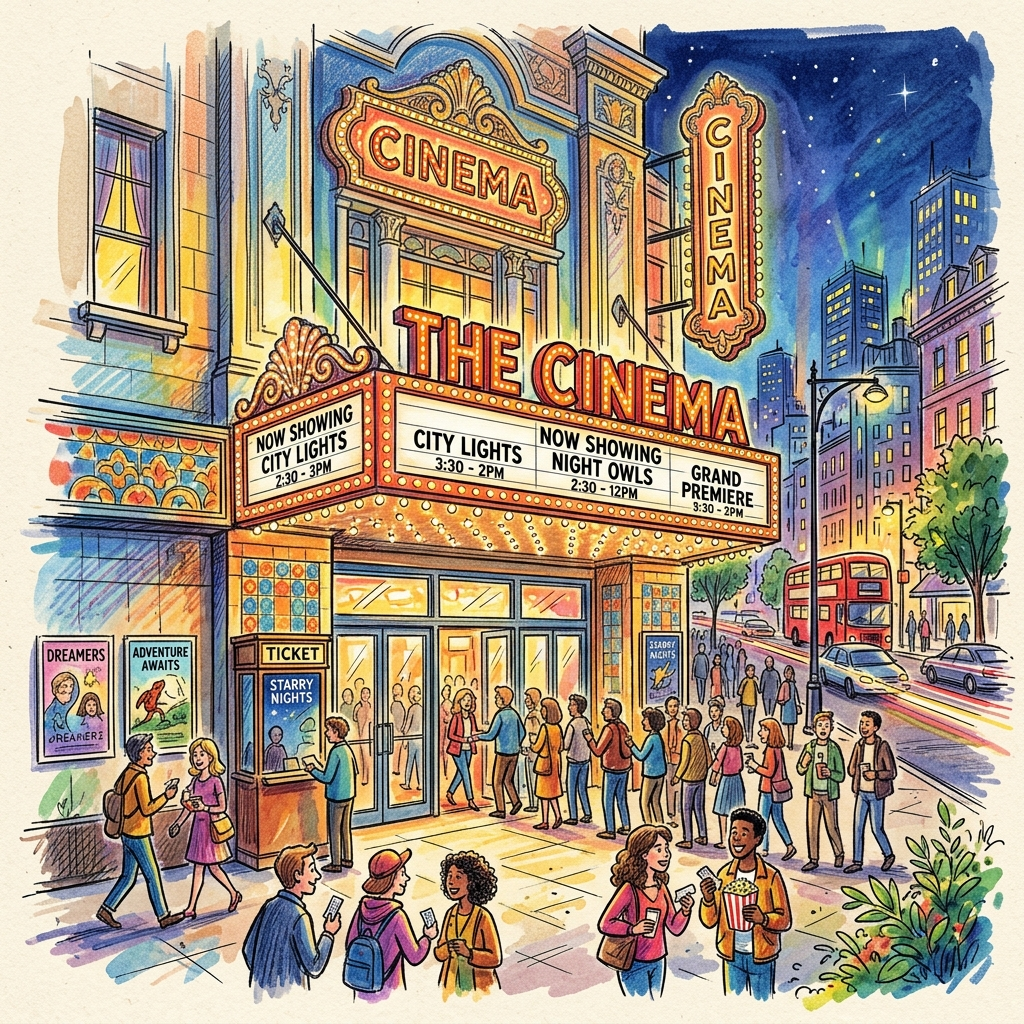
\includegraphics[width=0.85\linewidth]{vokab_300dpi/kino.png} \\
            \vspace{0.3cm}
    }}
    \vspace{0.4em}
    \textbf{\Large De Kino}\\
    \small\textit{(Le cinéma / The cinema)}
\end{minipage}
\hfill
\begin{minipage}[t]{0.48\textwidth}
    \centering
    \textbf{\Large Eng Tëlee}
    \vspace{0.4em}
    \framebox{\parbox{0.88\linewidth}{\centering
            \vspace{0.3cm}
            
\includegraphics[width=0.85\linewidth]{vokab_300dpi/telee.png} \\
            \vspace{0.3cm}
    }}
    \vspace{0.4em}
    \textbf{\Large D'Tëlee}\\
    \small\textit{(La télévision / The television)}
\end{minipage}
\end{noindent}

\vspace{2em}

\begin{noindent}
\begin{minipage}[t]{0.48\textwidth}
    \centering
    \textbf{\Large En Handy}
    \vspace{0.4em}
    \framebox{\parbox{0.88\linewidth}{\centering
            \vspace{0.3cm}
            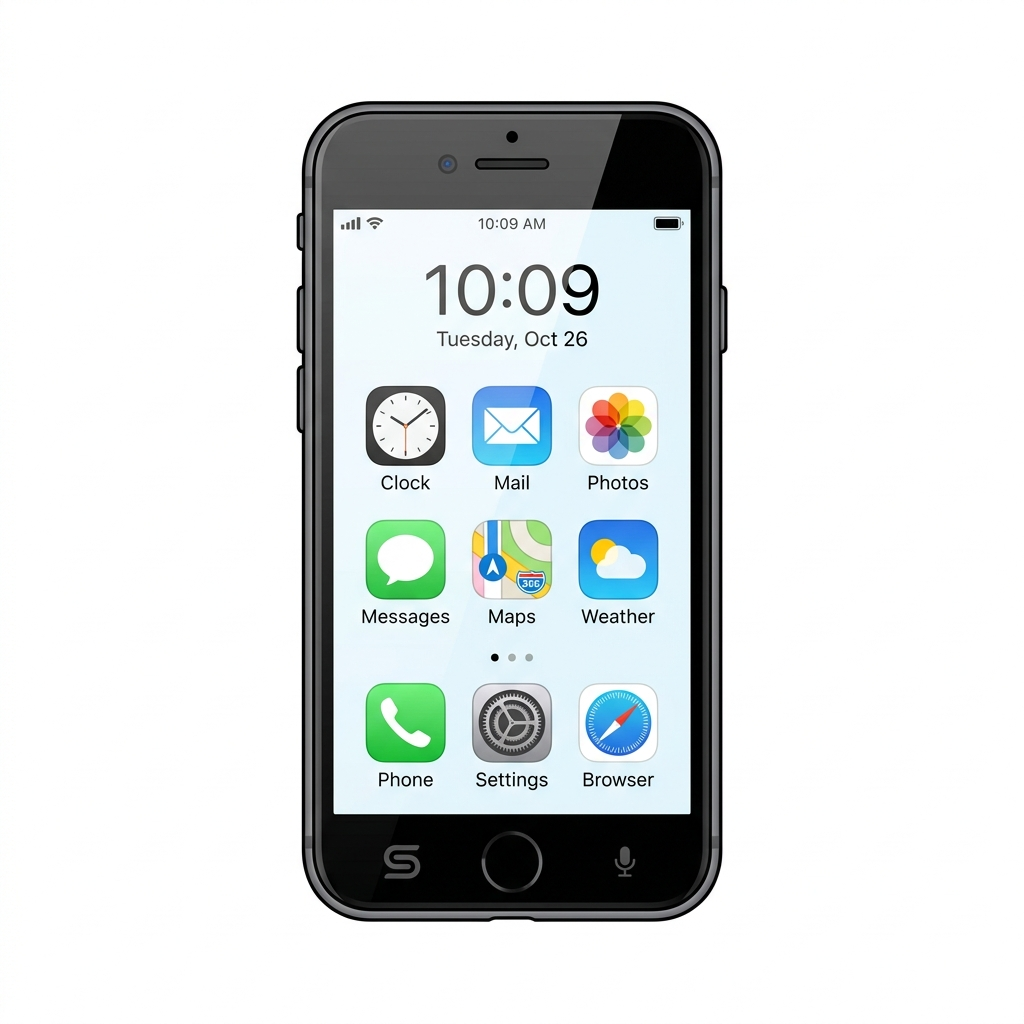
\includegraphics[width=0.85\linewidth]{vokab_300dpi/handy.png} \\
            \vspace{0.3cm}
    }}
    \vspace{0.4em}
    \textbf{\Large Den Handy}\\
    \small\textit{(Le téléphone / The smartphone)}
\end{minipage}
\hfill
\begin{minipage}[t]{0.48\textwidth}
    \centering
    \textbf{\Large E Computer}
    \vspace{0.4em}
    \framebox{\parbox{0.88\linewidth}{\centering
            \vspace{0.3cm}
            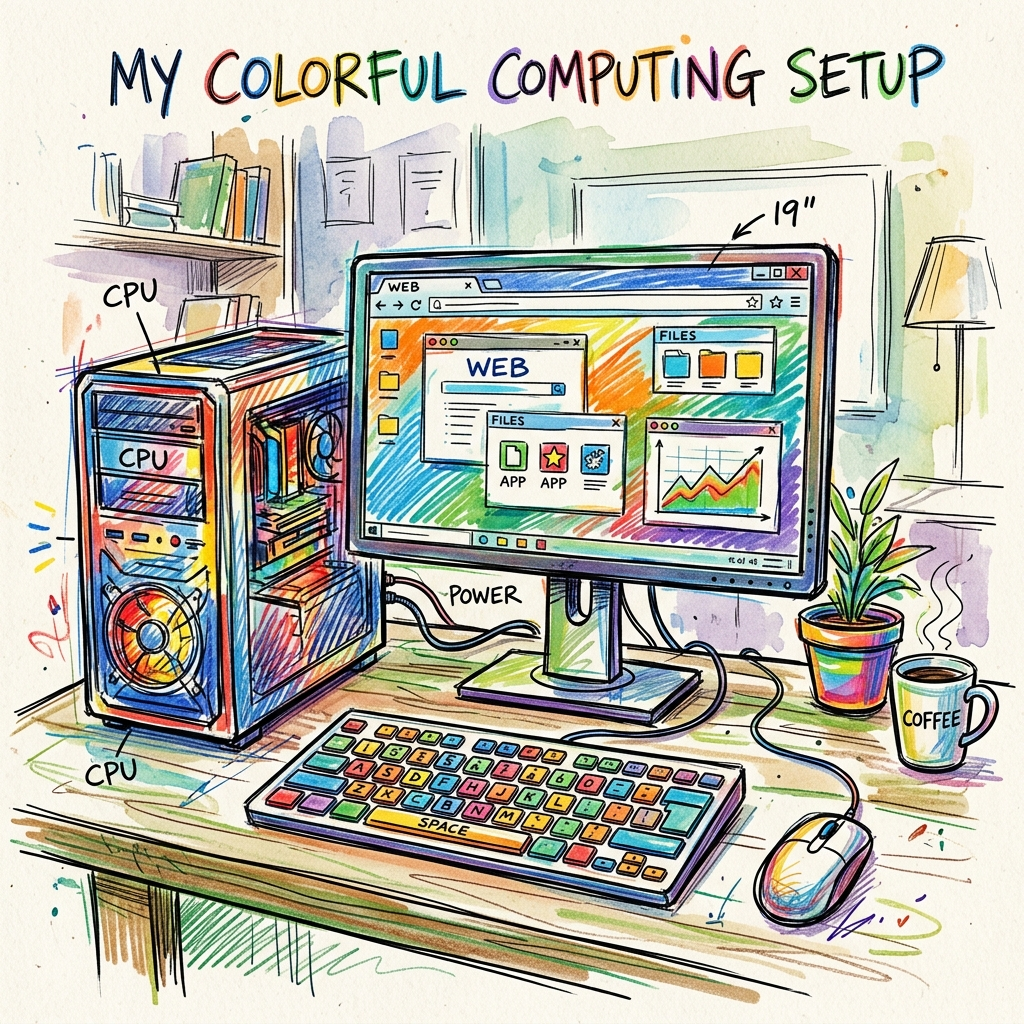
\includegraphics[width=0.85\linewidth]{vokab_300dpi/computer.png} \\
            \vspace{0.3cm}
    }}
    \vspace{0.4em}
    \textbf{\Large De Computer}\\
    \small\textit{(L'ordinateur / The computer)}
\end{minipage}
\end{noindent}
